% Copyright (c) 2008-2009 solvethis
% Copyright (c) 2010-2016,2018-2019,2021 Casper Ti. Vector
% Copyright (c) 2021 Kurapica
% Copyright (c) 2021 iofu728
% Local version.

%*********************************************************************
% iofu728-pkuthss: 北京大学研究生学位论文模板
% 2021/06/09 v1.0.0
%
% 重要提示:
%   1. 当前overleaf版符合2021研究生学位论文要求,可通过图书馆审核
%   2. 当前版本基于pkuthss v1.9.1
%   3. 请使用UTF-8编码,XeLaTeX方式编译
%   4. 请仔细阅读用户文档
%   5. 修改、使用、发布本文档类请务必遵循LaTeX Project Public License和知识共享4.0
%   6. 如有疑问github/iofu728/pkuthss上提问或联系作者@iofu728
%*********************************************************************

\documentclass[fontset=fandol,ugly]{pkuthss}
  % 学位论文模式  ugly    (默认打开,请保留)
  % 盲审模式      blind   (默认关闭)
  % 字体库       fontset
  %   auto | windows | windows@overleaf | mac | fandol | ubuntu | none
  % 除fandol,ubuntu外为商业字体,如需使用请遵循相应版权协议(需要已安装相应的字体)
  % fandol与windows效果相近,但字符库偏少,推荐使用(默认);
  % ubuntu字体效果偏差较大; 设为none时需自行配置字体集;
  % fandol与windows效果相近,但字符库偏少,推荐使用(默认);
  % ubuntu字体效果偏差较大;设为none时需自行配置字体集;

\usepackage[backend=biber,style=gb7714-2015]{biblatex}
  % 参考文献遵循GB/T 7714-2015标准,使用biblatex-gb7714-2015 宏包。
  % 此处使用顺序编码制,如使用著者-出版年制则更改为b7714-2015ay。

% 示例文档用包和设定,该段均可移除.
\usepackage{enumitem,fancyvrb}
\usepackage{booktabs,multirow,longtable,makecell} % 表格相关
\RecustomVerbatimEnvironment{Verbatim}{Verbatim}{frame = single, tabsize = 4, fontsize=\footnotesize}
\renewcommand{\v}[1]{\boldsymbol{#1}}
\newcommand\pkg[1]{\textsf{#1}}

% 参考文献边距字体
\setlength{\bibitemsep}{3bp}
\renewcommand*{\bibfont}{\zihao{5}\linespread{1.27}\selectfont}

\pkuthssinfo{
	cthesisname = {硕士学位论文},
 	thesiscover = {硕士研究生学位论文},
	ethesisname = {Master Thesis},
	ctitle = {基于XXXX的XXXX系统设计与实现},
	etitle = {Design and implementation of a XXXXX system based on XXXX},
	cauthor = {扎克·施耐德}, eauthor = {Zack Snyder},
	studentid = {180XXXXXXX},
	% 具体时间以教务为准,初稿3月,送审4月,答辩5月,最终6月。
	date = {\zhdigits{2021}\ \ 年\ \ \zhnumber{6}\ \ 月},
	school = {XXXXXX学院},
	cmajor = {XXXX}, emajor = {XXXX},
	direction = {XXXX},
	mentorlines = {2}, % 导师个数
	% 副教授 A.P. 讲师 Lec.
	cmentor = {XXX\ \ 教授\\YYY\ \ 教授}, ementor = {Prof.\ XXX and Prof.\ YYY},
	ckeywords = {A,B,C,D},
	ekeywords = {A,B,C,D},
	% 盲审模式参数, 需在documentclass增加blind
	blindid = {XXXXXXXXX}, discipline = {XXXX}
}
\addbibresource{thesis.bib}


\begin{document}
	\frontmatter
	\pagestyle{empty}
	\maketitle
	\cleardoublepage
	% 需替换门户版权声明pdf
	% Copyright (c) 2008-2009 solvethis
% Copyright (c) 2010-2017,2021 Casper Ti. Vector
% Copyright (c) 2021 iofu728
% All rights reserved.
%
% Redistribution and use in source and binary forms, with or without
% modification, are permitted provided that the following conditions are
% met:
%
% * Redistributions of source code must retain the above copyright notice,
%   this list of conditions and the following disclaimer.
% * Redistributions in binary form must reproduce the above copyright
%   notice, this list of conditions and the following disclaimer in the
%   documentation and/or other materials provided with the distribution.
% * Neither the name of Peking University nor the names of its contributors
%   may be used to endorse or promote products derived from this software
%   without specific prior written permission.
%
% THIS SOFTWARE IS PROVIDED BY THE COPYRIGHT HOLDERS AND CONTRIBUTORS "AS
% IS" AND ANY EXPRESS OR IMPLIED WARRANTIES, INCLUDING, BUT NOT LIMITED TO,
% THE IMPLIED WARRANTIES OF MERCHANTABILITY AND FITNESS FOR A PARTICULAR
% PURPOSE ARE DISCLAIMED. IN NO EVENT SHALL THE COPYRIGHT HOLDER OR
% CONTRIBUTORS BE LIABLE FOR ANY DIRECT, INDIRECT, INCIDENTAL, SPECIAL,
% EXEMPLARY, OR CONSEQUENTIAL DAMAGES (INCLUDING, BUT NOT LIMITED TO,
% PROCUREMENT OF SUBSTITUTE GOODS OR SERVICES; LOSS OF USE, DATA, OR
% PROFITS; OR BUSINESS INTERRUPTION) HOWEVER CAUSED AND ON ANY THEORY OF
% LIABILITY, WHETHER IN CONTRACT, STRICT LIABILITY, OR TORT (INCLUDING
% NEGLIGENCE OR OTHERWISE) ARISING IN ANY WAY OUT OF THE USE OF THIS
% SOFTWARE, EVEN IF ADVISED OF THE POSSIBILITY OF SUCH DAMAGE.

% 此处不用 \specialchap,因为学校要求目录不包括其自己及其之前的内容。
\chapter*{版权声明}
% 综合学校的书面要求及 Word 模版来看,版权声明页不用加页眉、页脚。
\thispagestyle{empty}

任何收存和保管本论文各种版本的单位和个人,
未经本论文作者同意,不得将本论文转借他人,
亦不得随意复制、抄录、拍照或以任何方式传播。
否则一旦引起有碍作者著作权之问题,将可能承担法律责任。

% 替换门户下载pdf
\begin{textblock}{1}(-0.8,-0.08)
  \colorbox{white}{
    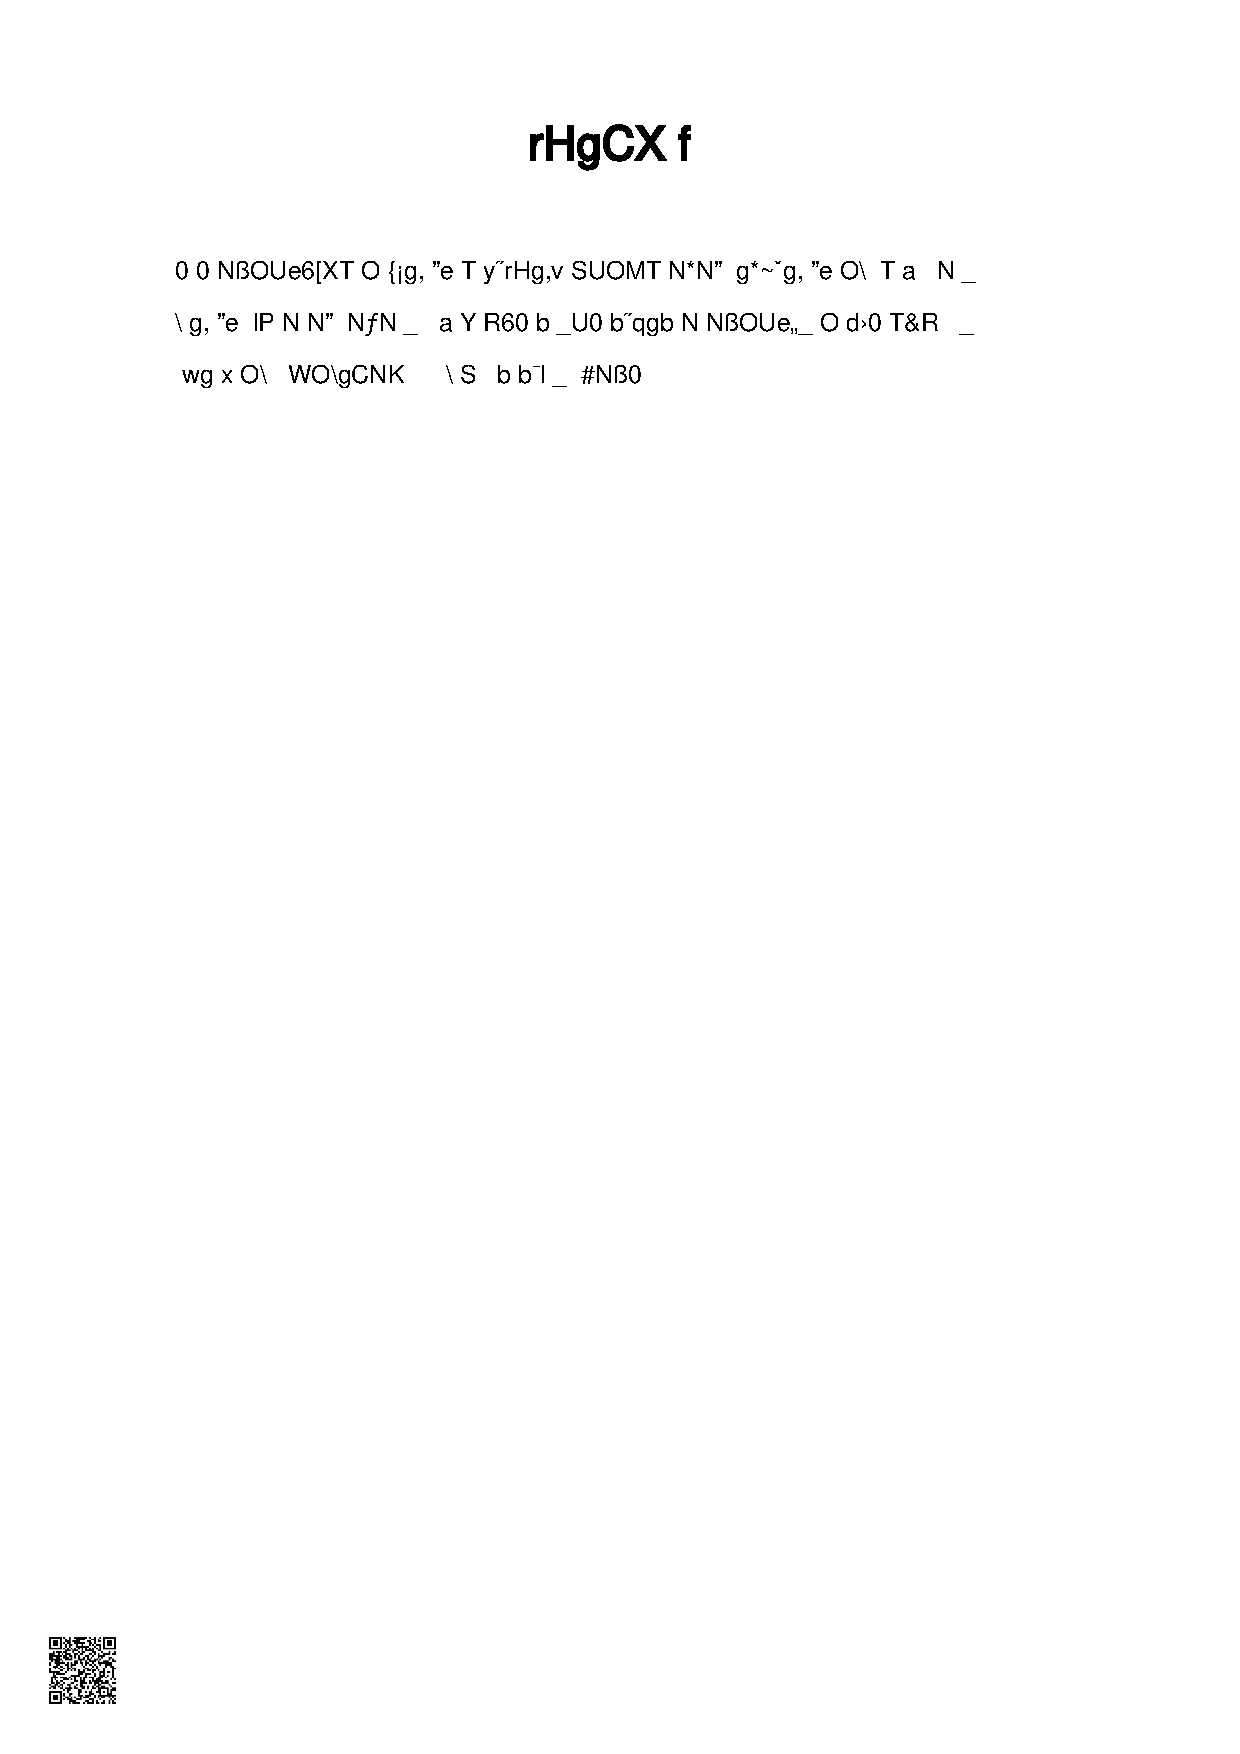
\includegraphics[height = 1.2448\textheight]{img/bqsm_180xxxxxxx.pdf}
  }
\end{textblock}


	\cleardoublepage
	\pagestyle{plain}
	\setcounter{page}{0}
	\pagenumbering{Roman}
	\begin{cabstract}
	中文摘要部分...
\end{cabstract}

\begin{eabstract}
    英文摘要部分...
\end{eabstract}

% vim:ts=4:sw=4

	\tableofcontents
	% 如有需要使用主要符号对照表
	\begin{denotation}

\item[$x,y,m,n,t$] 标量,通常为变量
\item[$K,L,D,M,N,T$] 标量,通常为超参数
\item[$x\in \mathbb{R}^{D}$] D维列向量
\item[$(x_1,\cdots,x_D)$] D维行向量
\item[$(x_1,\cdots,x_D)^T$ or $(x_1;\cdots;x_D)^T$]  D维行向量
\item[$\v A\in \mathbb{R}^{K\times D}$]  大小为$K\times D$的矩阵
\item[$x\in \mathbb{R}^{KD}$]  ($KD$)维的向量
\item[$\mathbb{M}_i$ or $\mathbb{M}_i(\v x)$]  第$i$列为$\v 1$(或者$\v x$),其余为$\v 0$的矩阵
\item[$diag(\v x)$]  对角矩阵,其对角元素为$\v x$
\item[$\v I_N$ or $I$]  ($N\times N$)的单位阵
\item[$diag(\v A)$]  列向量,其元素为$\v A$的对角元素
\item[$\v A \in \mathbb{R}^{D_1\times D_2\times \cdots \times D_K}$]  大小为$D_1\times D_2\times \cdots \times D_K$的张量
\item[$\{x^{(n)}\}^{N}_{n=1}$]  集合
\item[$\{(x^{(n)},y^{(n)})\}^{N}_{n=1}$]  数据集
\item[$\mathcal{N}(\v x;\mu,\sum)$]  变量$x$服从均值为$\mu$,方差为$\sum$的高斯分布

\end{denotation}

\footnotetext[1]{本符号对照表内容选自\citeauthor{qiu2020nndl}老师的《神经网络与深度学习》\cite{qiu2020nndl}一书。}

	\mainmatter
	\chapter{引论}
\label{chap:introduction}

本章为\iofupkuthss{}\footnote{\iofupkuthss{} 是基于\pkuthss{}~\cite{casper2011pkuthss}针对硕士研究生学位论文要求进行适配的\LaTeX{}文档类,符合北京大学硕士学位论文写作规范,并能通过图书馆审查。其官方仓库为\url{https://github.com/iofu728/pkuthss},当前版本\iofuversion。}文档类的示例文档,对硕士学位论文写作过程中常见用法和问题进行介绍说明。

\section{封面及pkuthssinfo相关}
\label{sec:cover-pkuthssinfo}

pkuthssinfo相关配置与\pkuthss{}原文档类完全一致,均为参数配置,可参考\pkuthss{}文档\footnote{\url{https://bbs.pku.edu.cn/attach/c8/3e/c83e980c93b838a3/pkuthss-bootstrap-0.1.7.pdf}}。
目前\iofupkuthss{}基于\pkuthss{} \iofubaseversion{}进行开发。

封面部分参考《北京大学研究生学位论文写作指南V2.0-2019》(以下简称写作指南)第1.1节中描述和《硕士论文模板2020》进行修改。

\begin{Verbatim}
\pkuthssinfo{
  cthesisname = {硕士学位论文},
  thesiscover = {硕士研究生学位论文},
  ethesisname = {Master Thesis},
  ctitle = {基于XXXX的XXXX系统设计与实现},
  etitle = {Design and implementation of a XXXXX system based on XXXX},
  cauthor = {扎克·施耐德}, eauthor = {Zack Snyder},
  studentid = {180XXXXXXX},
  % 具体时间以教务为准,初稿3月,送审4月,答辩5月,最终6月。
  date = {\zhdigits{2021}\ \ 年\ \ \zhnumber{6}\ \ 月},
  school = {XXXXXX学院},
  cmajor = {XXXX}, emajor = {XXXX},
  direction = {XXXX},
  mentorlines = {2}, % 导师个数
  % 副教授 A.P. 讲师 Lec.
  cmentor = {XXX\ \ 教授\\YYY\ \ 教授}, ementor = {Prof.\ XXX and Prof.\ YYY},
  ckeywords = {A,B,C,D},
  ekeywords = {A,B,C,D},
  % 盲审模式参数, 需在documentclass增加blind
  blindid = {XXXXXXXXX}, discipline = {XXXX}
}
\end{Verbatim}

\section{字体设定}
\label{sec:fontset}

本文档类提供五种默认字体设定分别为\verb|windows|,\verb|windows@overleaf|,\verb|mac|,\verb|ubuntu|,\verb|fandol|。
其中,默认情况,Overleaf平台下仅可使用\verb|fandol|,\verb|ubuntu|两种模式,\textbf{推荐使用}\verb|fandol|\textbf{模式(默认)}。
如遇字符不显示问题,可使用\verb|ubuntu|模式,或者自行收集上传所需的字体文件\verb|simsun.ttf|,\verb|simhei.ttf|,\verb|simfang.ttf|,\verb|simkai.ttf|至根目录并使用\verb|windows@overleaf|模式(注意文件名称和 版权问题),亦或者下载至本地windows环境使用\verb|windows|模式。详细可见第\ref{chap:related}章文档内容。

\section{版权声明与原创页}
\label{sec:copy-origin}

写作指南中要求各学生从校内门户或者从研究生院网站下载相应的文件进行签名后扫描替换或者直接替换。
\textbf{需要注意的是},门户生成的PDF文件未嵌入字体,其指定字体为华文宋体(即STSong)。
由于各个PDF预览器和操作系统预设的字体不同,导致呈现效果差异较大
(据不完全统计,Mac 端PDF Expert显示的是苹方简体,Chrome显示的是方正粗宋,而Acrobat显示的是AdobeSongStd,Windows端Edge显示的是方正悠黑,在这之中Acrobat字体效果最为接近)。
\textbf{请务必使用Acrobat进行打印,或者使用Overleaf平台生成的文件进行打印}
\footnote{由于样例中的PDF被编辑过,最终生成文件在不同PDF浏览器下仍然显示不同,使用门户下载文件生成则可以保持在不同PDF浏览器效果一致。}。

此外,写作指南中申明目录中需要保留原创页\footnote{对于这点部分人解读写作指南为目录中不需要,实际上写作指南第1.10节中声明,致谢(后记或说明)、学位论文原创性声明和授权使用说明是论文的最后两项内容,目录中和章平级。}。
本文使用\verb|textblock|和\verb|colorbox|宏包通过遮掩和覆盖的方式实现保留目录前提下的的PDF文件插入,其中参数按照PDF格式为A4进行调校,如有需要可以进行微调。

\begin{Verbatim}
    \begin{textblock}{1}(-0.8,-0.08)
    \colorbox{white}{
        \includegraphics[height = 1.2448\textheight]{文件路径}
    }
    \end{textblock}
\end{Verbatim}

此外在论文电子版制作过程中,需要替换原创页签名扫描件,使用相同方式即可。

\section{摘要部分}
\label{sec:abstract}

在\verb|\begin{cabstract}|和\verb|\begin{eabstract}|环境中进行书写。
如论文工作受到基金资助,需要在中文摘要第一页的页脚处标注:本研 究得到某某基金(编号:xxx)资助。

\section{目录}
\label{sec:directory}

按照写作指南和《硕士论文模板2020》进行调整,1)对章级增加点线;2)对间距和字体进行调整。

\section{主要符号对照表}
\label{sec:denotation}

参考\verb|chap/deno.tex|即可,在\verb|\begin{denotation}|环境下,使用\verb|\item[X] Y|分别表示符号及其说明。

已知问题: 符号处不能输入中括号$[$,$]$。

\section{图表相关}
\label{sec:table-figure}

\subsection{表格样例}
\label{sec:table-example}

一般学术论文需要使用三线表(如表~\ref{tab:example-table-basic}),需要依赖宏包\verb|booktabs|,使用\verb|\toprule|,\verb|\midrule|,\verb|\bottomrule|控制三线。
此外表序和表名位于表格的上方。
如果需要对表格内进行脚注,可通过\texttt{minipage}中嵌套\texttt{tabular}来实现,具体可参考Stack Overflow\footnote{\url{https://stackoverflow.com/questions/2888817/footnotes-for-tables-in-latex}}。

{\begin{longtable}[c]{c*{7}{r}}
\caption[续表]{续表样例表。}
\label{tab:example-table-continue}\\
\toprule[1.5pt]
 \multicolumn{1}{c}{年龄} & 性别 & \multicolumn{1}{c}{cp} & \multicolumn{1}{c}{静息血压} & \multicolumn{1}{c}{chol}
& \multicolumn{1}{c}{空腹血糖>} & \multicolumn{1}{c}{restecg} & \multicolumn{1}{c}{thalachh} \\
\multicolumn{1}{c}{(岁)} & & \multicolumn{1}{c}{胸痛型}&
\multicolumn{1}{c}{毫米汞柱}& \multicolumn{1}{c}{胆固醇}& \multicolumn{1}{c}{
   120 mg/dl}& 静息状态 & 最大心率 \\\midrule[1pt]
\endfirsthead
\multicolumn{8}{c}{续表~\thetable\hskip1em 续表样例表。}\\
\toprule[1.5pt]
 \multicolumn{1}{c}{年龄} & 性别 & \multicolumn{1}{c}{cp} & \multicolumn{1}{c}{静息血压} & \multicolumn{1}{c}{chol}
& \multicolumn{1}{c}{空腹血糖>} & \multicolumn{1}{c}{restecg} & \multicolumn{1}{c}{thalachh} \\
\multicolumn{1}{c}{(岁)} & & \multicolumn{1}{c}{胸痛型}&
\multicolumn{1}{c}{毫米汞柱}& \multicolumn{1}{c}{胆固醇}& \multicolumn{1}{c}{
   120 mg/dl}& 静息状态 & 最大心率 \\\midrule[1pt]
\endhead
\hline
\multicolumn{8}{r}{续下页}
\endfoot
\endlastfoot
63 & 1 & 3 & 145 & 233 & 1 & 0 & 150 \\
37 & 1 & 2 & 130 & 250 & 0 & 1 & 187 \\
41 & 0 & 1 & 130 & 204 & 0 & 0 & 172 \\
56 & 1 & 1 & 120 & 236 & 0 & 1 & 178 \\
57 & 0 & 0 & 120 & 354 & 0 & 1 & 163 \\
57 & 1 & 0 & 140 & 192 & 0 & 1 & 148 \\
56 & 0 & 1 & 140 & 294 & 0 & 0 & 153 \\
44 & 1 & 1 & 120 & 263 & 0 & 1 & 173 \\
52 & 1 & 2 & 172 & 199 & 1 & 1 & 162 \\
57 & 1 & 2 & 150 & 168 & 0 & 1 & 174 \\
54 & 1 & 0 & 140 & 239 & 0 & 1 & 160 \\
48 & 0 & 2 & 130 & 275 & 0 & 1 & 139 \\
49 & 1 & 1 & 130 & 266 & 0 & 1 & 171 \\
64 & 1 & 3 & 110 & 211 & 0 & 0 & 144 \\
\bottomrule[1.5pt]
\end{longtable}
\footnotesize 注:数据来源于Kaggle Heart Attack Analysis \& Prediction Data Set。}

如需要注明表格中数据来源,则可使用类似的方式,见表~\ref{tab:example-table-source-foot}。

\begin{table*}[htb]
    \centering
    \begin{minipage}[t]{0.55\linewidth} %
        \caption[表格脚注样例表]{表格脚注样例表。表名可通过中括号添加缩略名。}
        \label{tab:example-table-basic}
        \begin{small}
        \begin{tabular}{@{}lccccc@{}}
         \toprule[1.5pt]
         & \textbf{X} & \textbf{Y} & \textbf{Z} & \textbf{N} & \textbf{M} \\
         \midrule[1pt]
            默认        & 99.99 & 99.99 & 99.99 & 99.99\footnote{表格中的脚注1} & 99.99 \\
          \quad w/o X   & 99.99 & 99.99 & 99.99 & 99.99 & 99.99 \\
          \quad w/o Y   & 99.99 & 99.99 & 99.99 & 99.99 & 99.99 \\
          \quad w/o Z   & 99.99\footnote{表格中的脚注2} & 99.99 & 99.99 & 99.99 & 99.99 \\
          \quad w/o N   & 99.99 & 99.99 & 99.99 & 99.99 & 99.99 \\
          \quad w/o M   & 99.99 & 99.99 & 99.99 & 99.99 & 99.99 \\
          \bottomrule[1.5pt]
        \end{tabular}
        \end{small}
    \end{minipage}
\end{table*}

\begin{table*}[htbp]
   \centering
   \caption[数据来源注释表]{表格数据来源注释样例表。}
   \label{tab:example-table-source-foot}
   \begin{minipage}[t]{0.9\textwidth}
   \begin{small}
   \begin{tabular}{@{}l|ccc|ccc@{}}
   \toprule
   \multirow{2}{*}{\textbf{Model}} & \multicolumn{3}{c|}{\textbf{数据集A}} & \multicolumn{3}{c}{\textbf{数据集B}} \\ \cmidrule(l){2-7}
    & \textbf{指标a}(\%) & \textbf{指标b}(\%) & \textbf{指标c} & \textbf{指标a} (\%) & \textbf{指标b}(\%) & \textbf{指标c} \\ \midrule
      \citet{devlin2018bert}      &99.99  & 99.99  & 99.99  &99.99  & 99.99  & 99.99  \\
      \citet{yang2019xlnet}      &99.99  & 99.99  & 99.99  &99.99  & 99.99  & 99.99  \\
    \bottomrule
   \end{tabular}\\[6pt]
   \footnotesize 注:数据来源XXXXXX。\\
   \end{small}
   \end{minipage}
\end{table*}

当表格较大,不能在一页内打印时,可以“续表”的形式另页打印,可使用宏包\verb|longtable|实现,如表~\ref{tab:example-table-continue}。

\subsection{图片样例}
\label{sec:figure-example}

\begin{figure}[htb]
  \centering
  \subfloat[北京大学校徽]{
    \label{sfig:example-fig-logo-fig}
    
\includegraphics[height=2cm]{img/pku-fig-logo}}\hspace{4em}
  \subfloat[北京大学中文校名,依照北京大学标识管理办公室出具的北大标识使用基本规范进行使用]{
    \label{sfig:example-fig-logo-text}
    
\includegraphics[height=2cm]{img/pku-text-logo}}
  \caption{包含子图形的大图形}
  \label{fig:example-fig-subfloat}
\end{figure}

当需要插入多个子图的时候,可以选用宏包\verb|subfloat|,不推荐使用
\verb|subfigure| 和 \verb|subtable|。

若使用继承于\verb|subfigure|的宏包,例如\verb|subfloat|、\verb|subfigure|等,则可直接使用引用\verb|\ref{sfig:xxxx}|引用子图label,如图~\ref{sfig:example-fig-logo-fig}。
否则需要引用主图,再单独标注子图序号,以便符合学位论文要求。

此外,与表格相反,图序和图名需要位于图片的下方。
如果含有子图,每个子图需要具有相应的子图名。


如果需要并排使用两个独立的图形,分别编排图序,则可使用\verb|minipage|,如图~\ref{fig:example-fig-abreast-1}和图~\ref{fig:example-fig-abreast-2}。

\begin{figure}[htb]
\begin{minipage}{0.48\textwidth}
  \centering
  
\includegraphics[height=2cm]{img/pku-fig-logo}
  \caption{北京大学校徽}
  \label{fig:example-fig-abreast-1}
\end{minipage}\hfill
\begin{minipage}{0.48\textwidth}
  \centering
  
\includegraphics[height=2cm]{img/pku-text-logo}
  \caption{北京大学中文校名,依照北京大学标识管理办公室出具的北大标识使用基本规范进行使用}
  \label{fig:example-fig-abreast-2}
\end{minipage}
\end{figure}

\section{公式}
\label{sec:equation}

公式部分考虑到写作指南中无关于公式页的说明,并未做改动,使用通用\LaTeX{}规范即可。对于复杂公式需求,可使用\verb|amsmath|宏包结合Mathpix\footnote{\url{https://mathpix.com/}}等自动化识别工具。

\begin{multline*}
\int_a^b\biggl\{\int_a^b[f(x)^2g(y)^2+f(y)^2g(x)^2]
 -2f(x)g(x)f(y)g(y)\,dx\biggr\}\,dy \\
 =\int_a^b\biggl\{g(y)^2\int_a^bf^2+f(y)^2
  \int_a^b g^2-2f(y)g(y)\int_a^b fg\biggr\}\,dy
\end{multline*}

上述公式来源于\citeauthor{liu2003uncertain}的《不确定规划》\citet{liu2003uncertain}。

\section{参考文献}
\label{sec:bibtex}

参考文献根据写作指南使用\verb|gb7714-2015|bibstyle进行管理,具体引用命令与日常使用类似,\verb|\cite{}|,\verb|\citet{}|,\verb|\citeauthor{}|,具体用法见相应文档\footnote{\url{https://github.com/hushidong/biblatex-gb7714-2015}}。

例如\verb|\cite{devlin2018bert}|=\cite{devlin2018bert},\verb|\citeauthor{gut2013probability}|=\citeauthor{gut2013probability},...
相对于的bib文件的书写基本上直接用Google Scholar拷贝的BibTex即可,部分属性按提示进行微调。
\begin{Verbatim}
    \usepackage[backend=biber,bibstyle=gb7714-2015,citestyle=gb7714-2015]{biblatex}
\end{Verbatim}

\section{其他}
\label{sec:other}

正文不建议使用四级目录\verb|\subsubsection{}|。

本示例文档参考写作指南,《硕士论文模板2020》,《清华大学学位论文\LaTeX{}模板使用示例文档》和《\pkuthss{} 使用说明》进行书写。
遵循 \LaTeX{} Project Public License 和 Attribution 4.0 International (CC BY 4.0) 开源协议。

\section{与\pkuthss{} \iofubaseversion{}异同}

\textbf{格式方面:}

\begin{enumerate}
    \item ``关键词” + ``KEY WORDS” 非粗体
    \item ``题目” key 字号2号,value 字号1号
    \item ``姓名” key 字号小3
    \item 隐藏超链接
    \item 目录字体、样式(点线)、间距
    \item 调整表格索引、插图索引格式
\end{enumerate}

\textbf{功能方面:}

\begin{enumerate}
    \item 增加主要符号对照表
    \item 脚注从当前页开始标注
    \item 表格内脚注样式
    \item 子图引用格式
    \item 字体模式
    \item 简化blind模式下用户设定
    \item Windows 下中易宋体的粗体用假粗体替代
    \item 语言模式
\end{enumerate}

	\chapter{理论基础}
\label{chap:related}

本章对\pkuthss{}适配Overleaf平台的工作进行阐述和整理,希望对有兴趣了解和有修改相应需求的同学有所帮助。
本人才疏学浅,如有纰漏欢迎交流指正。

\def\XeLaTeX{
\leavevmode
\setbox0=\hbox{X\lower.5ex\hbox{\kern-.15em\reflectbox{E}}\kern-.1667em\LaTeX}%
\dp0=0pt\ht0=0pt\box0
}

\section{Overleaf适配存在的问题}
\label{sec:overleaf-problem}

Overleaf是一个开源在线实时协作\LaTeX{}编辑器,其\url{www.overleaf.com}托管版本是基于Ubuntu构建的。
Overleaf适配过程中遇到的问题不是\TeX{} Live版本\footnote{Overleaf托管版本目前支持2014-2020共8种\TeX{} Live版本。},也不是\TeX{}排班引擎/方式的问题\footnote{Overleaf托管版本目前支持\LaTeX{},pdf\LaTeX{},Lua\LaTeX{},\XeLaTeX{}四种编译方式。而\pkuthss{}是支持\XeLaTeX{}、\LaTeX{}+DVIPDFM$x$和pdf\LaTeX{}三种模式,本文选择\XeLaTeX{}编译方式进行适配。},
主要问题在于如何在Overleaf平台设置满足学位论文要求的字体配置。

\section{适配细节}
\label{sec:overleaf-detail}

\pkuthss{}适配Overleaf问题可追溯到Casper/pkuthss的\href{https://github.com/CasperVector/pkuthss/issues/28}{Issue\#28}\footnote{\url{https://github.com/CasperVector/pkuthss/issues/28}}。
事实上当时@lianze已经给出了正确的解决方案。

\subsection{\CTeX{}字库特点}
\label{sec:ctex-font}

\pkuthss{}使用\CTeX{}宏集进行中文排版,具体为文档类\verb|ctexbook|。
而默认情况下,\CTeX{}宏集根据编译方式和操作系统指定相应字库。
表~\ref{tab:ctex-font-select}中归纳了默认状态下各个操作系统和编译方式对应的字库使用策略。

由于本文选用了\XeLaTeX{}编译方式进行适配,而原始文档类\pkuthss{}使用的是Windows下\verb|ctex-fontset|设定,Overleaf托管版本基于Linux系统,两者区别在于原始文档类\pkuthss{}使用商用字体库(例如中易黑体、微软雅黑等),而Overleaf托管版本使用开源中文字体库Fandol、思源字体等。

原先\pkuthss{}在\verb|ctex-fontset-pkuthss.def|定义了使用的字体依赖,具体情况如下:
\begin{itemize}
    \item \verb|\songti|,中易宋体,作为默认中文字体使用,衬线字体,\verb|\textrm|;
    \item \verb|\heiti|,中易黑体,无衬线字体,\verb|\bfseries|,\verb|\textbf|和\verb|\textsf|;
    \item \verb|\fangsong|,中易仿宋,等宽字体,\verb|\texttt|;
    \item \verb|\kaishu|,中易楷体,\verb|\textit|;
    \item \verb|\lishu|, \verb|\youyuan|这两者在Linux下不存在,在windows、founder、macnew字库中才存在。原\pkuthss{}文档类中仅申明未使用。
\end{itemize}

\begin{table}[htbp]
\centering
\begin{minipage}[t]{\linewidth} %
\caption{\CTeX{} 宏集自动配置字体策略}
\label{tab:ctex-font-select}
\resizebox{\linewidth}{!}{
\begin{tabular}{*{5}{c}}
  \toprule
             & macOS Old\footnotemark[1]
             & macOS New\footnotemark[2]
             & Windows\footnotemark[3]
             & 其他\footnotemark[4] \\
  \midrule
  \XeLaTeX   & \makecell{\pkg{xeCJK}\\华文字库}
             & \makecell{\pkg{xeCJK}\\华文字库 + 苹方}
             & \makecell{\pkg{xeCJK}\\中易字库 + 微软雅黑}
             & \makecell{\pkg{xeCJK}\\Fandol 字库\footnotemark[5]} \\
  \cmidrule(lr){1-5}
  Lua\LaTeX\footnotemark[6]
             & \makecell{\pkg{LuaTeX-ja}\\华文字库}
             & \makecell{\pkg{LuaTeX-ja}\\华文字库 + 苹方}
             & \makecell{\pkg{LuaTeX-ja}\\中易字库 + 微软雅黑}
             & \makecell{\pkg{LuaTeX-ja}\\Fandol 字库} \\
  \cmidrule(lr){1-5}
  pdf\LaTeX
             & 不可用
             & 不可用
             & \makecell{\pkg{CJK} + \pkg{zhmetrics}\\中易字库 + 微软雅黑\footnotemark[7]}
             & 不可用 \\
  \cmidrule(lr){1-5}
  \makecell{\LaTeX{} + \\ DVIPDFM$x$}
             & 不可用
             & \makecell{\pkg{CJK} + \pkg{zhmetrics}\\华文字库 + 苹方}
             & \makecell{\pkg{CJK} + \pkg{zhmetrics}\\中易字库 + 微软雅黑\footnotemark[7]}
             & \makecell{\pkg{CJK} + \pkg{zhmetrics}\\Fandol 字库} \\
  \cmidrule(lr){1-5}
  \makecell{up\LaTeX{} + \\DVIPDFM$x$}
             & 不可用
             & \makecell{\pkg{zhmetrics-uptex}\\华文字库 + 苹方}
             & \makecell{\pkg{zhmetrics-uptex}\\中易字库 + 微软雅黑}
             & \makecell{\pkg{zhmetrics-uptex}\\Fandol 字库} \\
  \bottomrule
\end{tabular}
}
\footnotetext[1]{Yosemite (10.10) 及以前的 macOS 系统。}
\footnotetext[2]{El Capitan (10.11) 及以后的 macOS 系统。}
\footnotetext[3]{仅支持 Windows Vista 及以后的 Windows 操作系统。}
\footnotetext[4]{\CTeX{}将其他系统统一归为 Linux。}
\footnotetext[5]{由马起园、苏杰、黄晨成等人开发的开源中文字体,
     参见:\url{https://www.ctan.org/pkg/fandol}。}
\footnotetext[6]{Lua\LaTeX{} 编译时使用 \pkg{LuaTeX-ja} 宏包。}
\footnotetext[7]{微软雅黑字体并不总是有效,与选项 \pkg{zhmap} 的取值有关。}
\\[6pt]
\footnotesize 注:数据来源与\CTeX{}宏集手册v2.5.6。\\
\end{minipage}
\end{table}

\subsection{fontset 设定}
\label{sec:overleaf-fontset}

\iofupkuthss{}在\verb|documentclass|中增加fontset参数,并预设了5种字体模式(另外还有auto,nono两种自适应模式),将字体设置能力暴露给用户,从而解决跨端的字体适配问题。

查阅写作指南,其中说明中文字体使用宋体、仿宋和黑体,英文字体使用Times New Roman和\textsf{Arial},共五种字体,对楷体、隶书、幼圆等字体并未提及。

由于Overleaf托管版本只拥有开源字体版权\footnote{具体清单详见Overleaf字体说明文档\url{https://www.overleaf.com/learn/latex/Questions/Which_OTF_or_TTF_fonts_are_supported_via_fontspec\%3F}},无商用字体版权(例如中易字集)。

\begin{table}[htb]
  \centering
  \caption{\iofupkuthss{}预设的五种字体模式}
  \label{tab:ctex-fontset}
  \begin{minipage}[t]{0.55\linewidth} %
  \begin{tabular}{ccccc}
    \toprule
    & \option{windows}\footnote{与windows@overleaf模式相同} & \option{mac}    & \option{ubuntu} & \option{fandol} \\
    \midrule
    宋体 & 中易宋体         & 华文宋体        & 思源宋体        & Fandol 宋体     \\
    \heiti{黑体} & 中易黑体         & 华文黑体        & 思源黑体        & Fandol 黑体     \\
    \fangsong{仿宋} & 中易仿宋         & 华文仿宋        & Fandol 仿宋     & Fandol 仿宋     \\
    \bottomrule
  \end{tabular}
  \end{minipage}
\end{table}

本文档类申明的5种字体模式\verb|fontset|对应使用字体情况如表~\ref{tab:ctex-fontset}所示。
其中,\verb|windows|和\verb|mac|模式为商业字体。默认情况下,不能在Overleaf平台上使用。而\verb|fandol|和\verb|ubuntu|模式为开源字体,可在Overleaf平台上使用。

而对于中文字体,不同种类的字体实现细节存在细微差异,所对应的字符数也不同,对于极生僻词开源字体可能会出现显示异常的情况,如垚y\'ao,\verb|fandol|模式下不可见。
但考虑到版权问题和字体效果,\textbf{Overleaf平台中仍然推荐使用}\verb|fandol|\textbf{模式}。
如在使用中发现较多字符不显示,可考虑使用\verb|ubuntu|模式,或者自行收集上传\verb|simsun.ttf|,\verb|simhei.ttf|,\verb|simfang.ttf|,\verb|simkai.ttf|至根目录并使用\verb|windows@overleaf|模式(注意文件名称和版权问题),亦或者下载至本地windows环境使用\verb|windows|模式。

为支持文档类的fontset设定能力,使用宏包\verb|kvsetkeys|,\verb|kvdefinekeys|,\verb|kvoptions|对key的默认值,可选范围进行管理。

\subsection{编码方式}
\label{sec:overleaf-encoding}

由于使用\XeLaTeX{}编译时,\CTeX{}宏集强制使用UTF-8编码,相对应的包括\verb|.def|文件、所有\verb|*.tex|文件均应该使用UTF-8编码方式进行编码。

\subsection{粗体设定}

由于Windows 下中易宋体无粗体实现,原文档类\pkuthss{}对于宋体的粗体\verb|\textbf{}|使用中易黑体替代,本文档类\iofupkuthss{}则依照Windows惯常设定,使用对应字体的假粗体作为粗体\verb|\textbf{}|。

	\chapter{Model 1}
\label{chap:model1}

第三章部分...

	\chapter{Model 2}
\label{chap:model2}

第四章部分...
	\chapter{Model 3}
\label{chap:model3}

第五章部分...
	\chapter{总结和展望}
\label{chap:conclusion}

第六章部分...

    
    \appendix
    \printbibliography[heading = bibintoc]
    % 如有需要使用研究生成果页
    \def\cpublication{攻读硕士期间发表的论文及其他成果}

\renewcommand{\bibname}{\cpublication}
\begin{thebibliography}{9}{
    \zihao{5}
    \bibitem{publish}
    \textbf{扎克·施耐德}, XXX XXX, et al. XXXX Title[C/OL]//III H D, SINGH A. Proceedings of Machine Learning Research: Proceedings of the 37th International Conference on Machine Learning: vol. 119. [S.l.]: PMLR, 2020: XXXX-XXXX. http://proceedings.ml r.press/XXXX.html.(一作,CCF-A)
  }\end{thebibliography}
\addcontentsline{toc}{chapter}{\cpublication}


	\backmatter
	\chapter{致谢}

致谢部分...

	% 需替换门户原创页pdf/扫描pdf
	% Copyright (c) 2008-2009 solvethis
% Copyright (c) 2010-2017,2021 Casper Ti. Vector
% Copyright (c) 2021 Kurapica
% Copyright (c) 2021 iofu728
% All rights reserved.
%
% Redistribution and use in source and binary forms, with or without
% modification, are permitted provided that the following conditions are
% met:
%
% * Redistributions of source code must retain the above copyright notice,
%   this list of conditions and the following disclaimer.
% * Redistributions in binary form must reproduce the above copyright
%   notice, this list of conditions and the following disclaimer in the
%   documentation and/or other materials provided with the distribution.
% * Neither the name of Peking University nor the names of its contributors
%   may be used to endorse or promote products derived from this software
%   without specific prior written permission.
%
% THIS SOFTWARE IS PROVIDED BY THE COPYRIGHT HOLDERS AND CONTRIBUTORS "AS
% IS" AND ANY EXPRESS OR IMPLIED WARRANTIES, INCLUDING, BUT NOT LIMITED TO,
% THE IMPLIED WARRANTIES OF MERCHANTABILITY AND FITNESS FOR A PARTICULAR
% PURPOSE ARE DISCLAIMED. IN NO EVENT SHALL THE COPYRIGHT HOLDER OR
% CONTRIBUTORS BE LIABLE FOR ANY DIRECT, INDIRECT, INCIDENTAL, SPECIAL,
% EXEMPLARY, OR CONSEQUENTIAL DAMAGES (INCLUDING, BUT NOT LIMITED TO,
% PROCUREMENT OF SUBSTITUTE GOODS OR SERVICES; LOSS OF USE, DATA, OR
% PROFITS; OR BUSINESS INTERRUPTION) HOWEVER CAUSED AND ON ANY THEORY OF
% LIABILITY, WHETHER IN CONTRACT, STRICT LIABILITY, OR TORT (INCLUDING
% NEGLIGENCE OR OTHERWISE) ARISING IN ANY WAY OUT OF THE USE OF THIS
% SOFTWARE, EVEN IF ADVISED OF THE POSSIBILITY OF SUCH DAMAGE.

{
\ctexset{section = {
format+ = {\centering}, beforeskip = {40bp}, afterskip = {15bp}
}}
\specialchap{北京大学学位论文原创性声明和使用授权说明}

% 学校书面要求本页面不要页码,但在给出的 Word 模版中又有页码。
% 此处以学校书面要求为准。
\thispagestyle{empty}

% 替换扫描pdf,去除includegraphics前注释
\begin{textblock}{1}(-0.8,-0.08)
  \colorbox{white}{
    
\includegraphics[height = 1.2448\textheight]{img/lwsm_180xxxxxxx.pdf}
  }
\end{textblock}
}


\end{document}

% vim:ts=4:sw=4